% !TEX root = ../review.tex
\begin{frame}
\frametitle{OPTIMA: Общие сведения}


\end{frame}

\begin{frame}
\frametitle{OPTIMA: Алгоритм}

Этапы выравнивания:
\begin{itemize}
  \item Поиск стартовых мест (сидов) для начала выравнивания
  \item Парное выравнивание карты с референсом
  \item Определение значимых выравниваний
  \item Объединение пересекающихся выравниваний
\end{itemize}

\end{frame}

\begin{frame}
\frametitle{OPTIMA: Композитные сиды}
Композитные сиды:
\begin{figure}
  \centering
  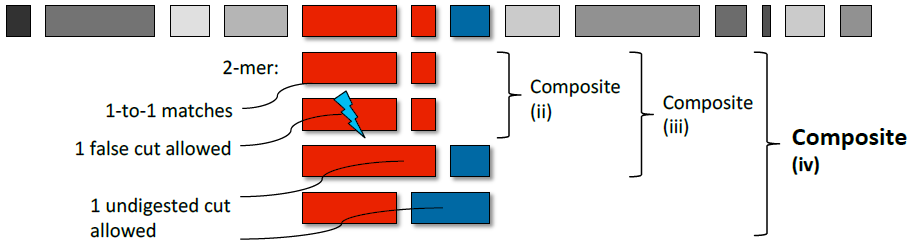
\includegraphics[width = 0.9\textwidth]{optima/composite_seeds}
\end{figure}
Множество фрагментов $o_k$, $o_{k + 1}$, $ \dots$, $o_{s}$ возможно
совпадает с множеством фрагментов $r_l$, $r_{l+1}$, $\dots$, $r_{t}$ :
\begin{gather}
\frac{\bigg|\sum\limits_{i = k}^s o_i - \sum\limits_{j = l}^t r_i \bigg|}{\sqrt{\sum\limits_{j = l}^t\sigma_j^2}} \le C_{\sigma}
\label{eq:feasible_match}
\end{gather}

\end{frame}

\begin{frame}
\frametitle{OPTIMA: Поиск стартовых сидов}
Алгоритм поиска сидов для выравнивания:
\begin{itemize}
  \item По референсу строятся композитные сиды и сортируются по первому элементу
  \item У карты берётся произвольный сид, по которому будем искать множество подходящих(\ref{eq:feasible_match}) локаций в референсе
  \item Бинарным поиском (по первому элементу) ищем множество подходящих сидов в референсе
  \item Далее линейно проверяем и оставляем только те, которые удовлетворяют (\ref{eq:feasible_match})
\end{itemize}
\end{frame}

\begin{frame}
\frametitle{OPTIMA: Парное выравнивание карты с референсом}

\end{frame}

\begin{frame}
\frametitle{OPTIMA: Определение значимости выравнивания}
Пусть $a$ - выравнивание из множества выравниваний $\mathcal{A}$
\begin{gather*}
Z-score(a \in \mathcal{A}, f) = \frac{f_{a} - Mean(f_{\mathcal{A}})}{SD(f_{\mathcal{A}})}
\end{gather*}
где $f$ - характеристика выравнивания.\\
 Тогда статистическая значимость выравнивания:
\begin{align*}
  \vartheta (a \in \mathcal{A}) = Z-score( & -Z-score(a, \#matches) \\
  & + Z-score(a, \#cuterrors) \\
  & + Z-score(a, WHT(\chi^2, \#matches))) \\
\end{align*}
\[\text{где } WHT(\chi^2, \#matches) = \frac{\sqrt[3]{\frac{\chi^2}{\#matches}} - \big(1 - \frac{1}{9} \frac{2}{\#matches}\big)}{\sqrt{\frac{1}{9} \frac{2}{\#matches}}}\]
\end{frame}

\begin{frame}
\frametitle{OPTIMA: Объединение пересекающихся выравниваний}

\end{frame}
